\documentclass[11pt]{article}

% Change "review" to "final" to generate the final (sometimes called camera-ready) version.
% Change to "preprint" to generate a non-anonymous version with page numbers.
\usepackage[review]{acl}

% Standard package includes
\usepackage{times}
\usepackage{latexsym}

\usepackage{polyglossia}

\setotherlanguage{bengali}
\newfontfamily\bengalifont[Script=Bengali]{Noto Serif Bengali}

\usepackage{array}
\usepackage{float}
\usepackage{amsmath}

% For proper rendering and hyphenation of words containing Latin characters (including in bib files)
\usepackage[T1]{fontenc}
% For Vietnamese characters
% \usepackage[T5]{fontenc}
% See https://www.latex-project.org/help/documentation/encguide.pdf for other character sets

% This assumes your files are encoded as UTF8
\usepackage[utf8]{inputenc}

% This is not strictly necessary, and may be commented out,
% but it will improve the layout of the manuscript,
% and will typically save some space.
\usepackage{microtype}

% This is also not strictly necessary, and may be commented out.
% However, it will improve the aesthetics of text in
% the typewriter font.
\usepackage{inconsolata}

%Including images in your LaTeX document requires adding
%additional package(s)
\usepackage{graphicx}

% If the title and author information does not fit in the area allocated, uncomment the following
%
%\setlength\titlebox{<dim>}
%
% and set <dim> to something 5cm or larger.

\title{From Words to Images: Bangla Political Bias Detection via Multimodal Deep Learning with Cross-Attention and Fusion Strategies}

% Author information can be set in various styles:
% For several authors from the same institution:
% \author{Author 1 \and ... \and Author n \\
%         Address line \\ ... \\ Address line}
% if the names do not fit well on one line use
%         Author 1 \\ {\bf Author 2} \\ ... \\ {\bf Author n} \\
% For authors from different institutions:
% \author{Author 1 \\ Address line \\  ... \\ Address line
%         \And  ... \And
%         Author n \\ Address line \\ ... \\ Address line}
% To start a separate ``row'' of authors use \AND, as in
% \author{Author 1 \\ Address line \\  ... \\ Address line
%         \AND
%         Author 2 \\ Address line \\ ... \\ Address line \And
%         Author 3 \\ Address line \\ ... \\ Address line}

\author{Meherunnesa Hossain Ibnath \\
  Ahsanullah University of Science and Technology / Dhaka, Bangladesh\\
  \texttt{meherunnesa.ibnath20@gmail.com} \\\And
  Second Author \\
  Affiliation / Address line 1 \\
  Affiliation / Address line 2 \\
  Affiliation / Address line 3 \\
  \texttt{email@domain} \\}

%\author{
%  \textbf{First Author\textsuperscript{1}},
%  \textbf{Second Author\textsuperscript{1,2}},
%  \textbf{Third T. Author\textsuperscript{1}},
%  \textbf{Fourth Author\textsuperscript{1}},
%\\
%  \textbf{Fifth Author\textsuperscript{1,2}},
%  \textbf{Sixth Author\textsuperscript{1}},
%  \textbf{Seventh Author\textsuperscript{1}},
%  \textbf{Eighth Author \textsuperscript{1,2,3,4}},
%\\
%  \textbf{Ninth Author\textsuperscript{1}},
%  \textbf{Tenth Author\textsuperscript{1}},
%  \textbf{Eleventh E. Author\textsuperscript{1,2,3,4,5}},
%  \textbf{Twelfth Author\textsuperscript{1}},
%\\
%  \textbf{Thirteenth Author\textsuperscript{3}},
%  \textbf{Fourteenth F. Author\textsuperscript{2,4}},
%  \textbf{Fifteenth Author\textsuperscript{1}},
%  \textbf{Sixteenth Author\textsuperscript{1}},
%\\
%  \textbf{Seventeenth S. Author\textsuperscript{4,5}},
%  \textbf{Eighteenth Author\textsuperscript{3,4}},
%  \textbf{Nineteenth N. Author\textsuperscript{2,5}},
%  \textbf{Twentieth Author\textsuperscript{1}}
%\\
%\\
%  \textsuperscript{1}Affiliation 1,
%  \textsuperscript{2}Affiliation 2,
%  \textsuperscript{3}Affiliation 3,
%  \textsuperscript{4}Affiliation 4,
%  \textsuperscript{5}Affiliation 5
%\\
%  \small{
%    \textbf{Correspondence:} \href{mailto:email@domain}{email@domain}
%  }
%}

\begin{document}
\maketitle
\begin{abstract}
Detecting political bias in news is essential for understanding public discourse and combating misinformation. In this paper, we introduce a multimodal deep learning architecture for Bangla political bias detection that leverages textual embeddings from Bangla-BERT and visual embeddings from ViT with a cross-attention-based fusion approach. Other fusion approaches, such as concatenation, summation, averaging, and multimodal factorized bilinear (MFB) fusion, are also considered. We curated a Bangla political dataset with paired images and texts labeled for bias. Experiments with stratified 5-fold cross-validation show that the cross-attention hybrid model outperforms other fusion techniques, achieving an accuracy of 63.2\%. Our results highlight the effectiveness of cross-attention in fusing heterogeneous modalities, establishing a benchmark for Bangla multimodal political bias detection. The cross-attention mechanism provides insights into the interaction between textual and visual modalities, highlighting potential areas where alignment between modalities may be improved.
\end{abstract}


\section{Introduction}

Political bias in news has become a critical challenge in the digital information ecosystem, influencing public opinion and democratic discourse. Detecting such bias is particularly important for low-resource languages like Bangla, where linguistic resources and annotated datasets remain limited. Although prior studies have shown progress in text-based political bias detection \citep{arman2025bengali, lia2025read} and multilingual multimodal frameworks \citep{bernard2025multimodal, thapa2025multimodal, mitra2026breaking}, several research gaps still exist. Notably, multimodal Bangla political bias datasets are scarce, fusion strategies for combining textual and visual features are underexplored, architectures jointly modeling sequential and visual representations are limited, and class-imbalance-aware loss functions are rarely utilized.

To address these limitations, we propose a multimodal framework for Bangla political bias detection that integrates Bangla-BERT for textual encoding and Vision Transformer (ViT) for visual feature extraction. The framework evaluates multiple feature-level fusion strategies, including cross-attention, concatenation, factorized bilinear fusion, summation, and averaging. Furthermore, class-weighted focal loss is employed to handle label imbalance and improve minority class prediction. By leveraging transformer-based models and effective fusion mechanisms, the proposed approach captures complementary information from both modalities, enabling more robust bias detection in multimedia political content.

Our contributions of this work are threefold. First, we introduce a transformer-based multimodal framework for Bangla political bias detection. Second, we provide a comparative analysis of different fusion strategies and examine the effectiveness of class-weighted focal loss in addressing label imbalance. Third, we conduct a comprehensive benchmark evaluation using five-fold cross-validation, reporting accuracy, precision, recall, and F1-score, along with confusion matrices and ROC curves for interpretability. Overall, this study establishes a strong benchmark for multimodal Bangla bias detection and offers practical insights for extending multimodal bias detection to other low-resource languages, building upon prior English and multilingual studies \citep{bernard2025multimodal, thapa2025multimodal, mohiuddin2025memeguard}.


\section{Related Work}

Political bias detection has been widely studied across textual, visual, and multimodal content. This section reviews prior research and identifies key gaps addressed by our work, with a particular focus on low-resource languages such as Bangla.

\subsection{Multimodal Political Bias and Fake News Detection}
Several studies have explored multimodal approaches for political bias and misinformation detection. Bernard et al. \citep{bernard2025multimodal} combined BERT, CLIP, and Vision Transformers for bias detection and neutralization in English news. Thapa et al. \citep{thapa2025multimodal} showed that CLIP-based and parameter-efficient fusion models outperform unimodal approaches in meme-based hate and stance detection. Li et al. \citep{li2025survey} surveyed multimodal fake news detection methods, emphasizing cross-modal interaction and alignment. Mitra et al. \citep{mitra2026breaking} proposed a context-aware multimodal framework for ideological bias detection in English news. 

\subsection{Bangla Political Text Analysis}
Text-only political bias and sentiment analysis in Bangla has received increasing attention. Arman et al. \citep{arman2025bengali} evaluated transformer-based models for Bangla political sentiment, reporting strong performance on textual data. Lia et al. \citep{lia2025read} introduced the first benchmark dataset for Bangla political bias detection, highlighting challenges in identifying neutral and subtle biases. Das et al. \citep{das2025datasets} and Aupi et al. \citep{aupi2025wonbias} analyzed identity-based and gender bias in Bangla NLP systems, revealing persistent low-resource challenges. Agrawal et al. \citep{agrawal2022hindi} demonstrated transformer-based bias detection for Hindi, indicating the feasibility of low-resource fine-tuning. 

\subsection{Multimodal Approaches in Low-Resource Languages}
Recent efforts have extended multimodal learning to low-resource settings. Mohiuddin et al. \citep{mohiuddin2025memeguard} introduced MemeGuard, a Bengali multimodal propaganda dataset, demonstrating improved performance through adaptive fusion of BanglaBERT and CLIP. Afroze et al. \citep{afroze2026mulmosent} proposed MulMoSenT, employing cross-attention between text and images for sentiment analysis in low-resource languages. Vu \citep{vu2017politicalbias} explored early MLP-based political bias detection using word embeddings. 

\subsection{Cross-Language and news Bias Analysis}
Political bias detection has also been studied in cross-lingual and news contexts. Wang et al. \citep{wang2025mediabias} developed a real-time media bias detector for English news. Yang and Menczer \citep{yang2025llmcredibility} exposed systematic bias in LLM-based credibility assessments. Purohit et al. \citep{purohit2025mediasentiment}, Yenkikar et al. \citep{yenkikar2022sentinet}, and Ness et al. \citep{ness2023data} analyzed long-term media bias using deep learning methods. Studies by Afroze et al. \citep{afroze2026mulmosent} and Agrawal et al. \citep{agrawal2022hindi} further demonstrate the applicability of transformer models in low-resource and news domains.


Overall, while multimodal and transformer methods perform well in high-resource languages, Bangla political bias detection remains underexplored. Prior work largely focuses on text-only analysis, English datasets, or simple fusion strategies. Our study addresses these gaps by introducing a cross-attention-based multimodal framework for Bangla, evaluating multiple fusion techniques, and using class-imbalance-aware loss functions for robust bias detection.

\section{Dataset Description}\label{sec:dataset}

\subsection{Data Collection}
We construct a multimodal Bangla political bias dataset comprising paired text--image news articles collected from major Bangla news platforms, including BBC Bangla, Prothom Alo, Jugantor, The Daily Star, Jago News, and Kaler Kantho. Each instance includes a headline, a corresponding image, publication metadata (date, source, and newspaper), and political bias annotations. The initial dataset contained 200 samples; after removing duplicates and visually redundant images, 198 instances remain. Each sample is labeled into one of three political bias categories: Govt Critique (0), Neutral (1), and Govt Leaning (2). The final dataset exhibits class imbalance, as summarized in Table~\ref{tab:class_distribution} and illustrated in Figure~\ref{fig:class_distribution}. Although the dataset provides a balanced representation of classes, its relatively small size (N=198) may limit the generalizability of deep learning models and increase the risk of overfitting.

\begin{table}[H]
\centering
\caption{Distribution of Political Bias Labels in the Cleaned Dataset}
\label{tab:class_distribution}
\begin{tabular}{|c|c|}
\hline
\textbf{Political Bias} & \textbf{Count} \\
\hline
Govt Critique & 103 \\
Neutral & 53 \\
Govt Leaning & 42 \\
\hline
\end{tabular}
\end{table}


\begin{figure}[h]
    \centering
    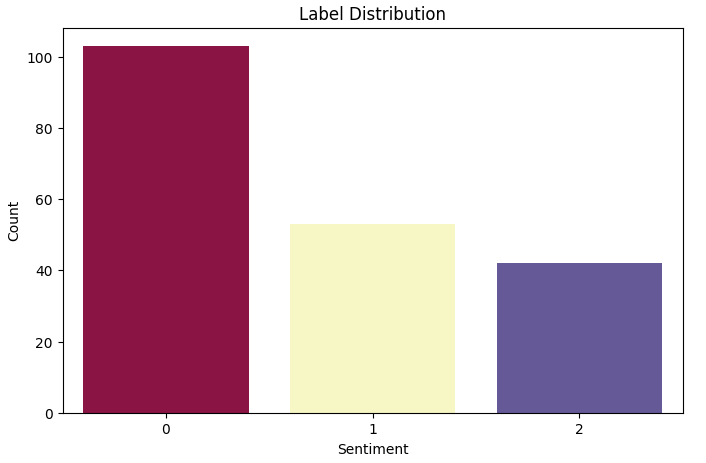
\includegraphics[width=0.9\linewidth]{class_dis.png}
    \caption{Class distribution of the cleaned Bangla multimodal political bias dataset.}
    \label{fig:class_distribution}
\end{figure}


\subsection{Data Preprocessing}

\subsubsection{Text Preprocessing}
We apply a Bangla-specific preprocessing pipeline to reduce noise and ensure linguistic consistency. This includes removing URLs, hashtags, and HTML tags; Unicode normalization (NFKC); filtering non-Bangla characters; converting emojis to textual descriptions; and normalizing whitespace and line breaks. 


\subsubsection{Text Augmentation}
To address class imbalance, text-only data augmentation is applied to minority classes while preserving semantic meaning. Techniques include synonym replacement using curated Bangla synonym sets, random word swapping and deletion, and controlled word insertion. Augmentation continues until each class reaches 104 samples. To prevent data leakage, augmentation is applied only on the training folds within each cross-validation split, ensuring no augmented samples appear in validation data. Since augmentation is applied only to textual data, multimodal models may receive uneven modality enhancement. This could influence performance comparisons and is a limitation of the current setup.

\subsubsection{Image Preprocessing}
For the visual modality, images smaller than $100 \times 100$ pixels are discarded, and all remaining images are converted to RGB format. Near-duplicate images are removed using perceptual hashing (pHash). Images are then resized with aspect ratio preservation and padded to $256 \times 256$ pixels for compatibility with the Vision Transformer (ViT). No image augmentation is applied; instead, class imbalance is handled during training using class-weighted loss functions to avoid introducing artificial visual artifacts.


\begin{figure*}[h]
    \centering
    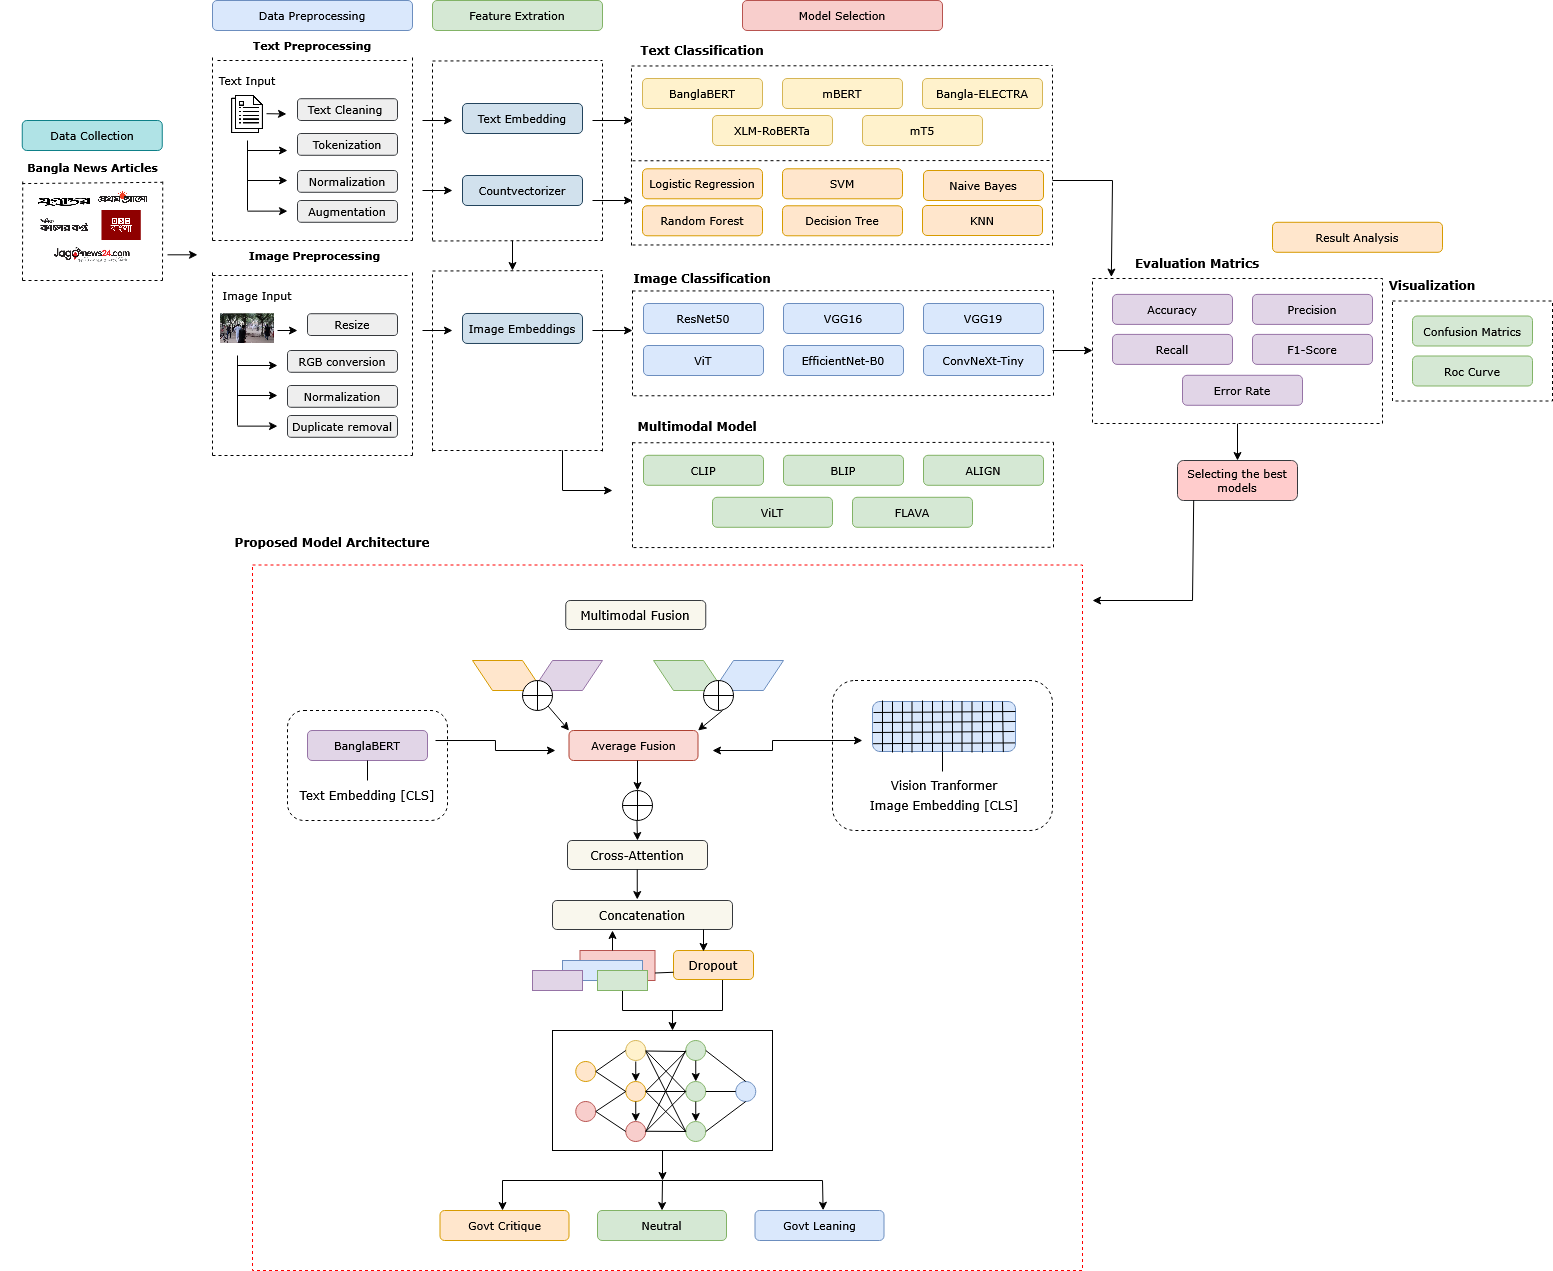
\includegraphics[width=1\linewidth]{method1.png}
    \caption{Proposed framework for Bangla political news bias detection.}
    \label{fig:multimodal_pipeline}
\end{figure*}


\section{Methodology}

This study proposes a framework for Bangla political bias detection using textual, visual, and multimodal data. We evaluate classical ML models, transformer-based models, and six multimodal architectures with different fusion strategies and loss functions. Dataset construction and preprocessing are detailed in Section~\ref{sec:dataset} and class weights to handle label imbalance. The dataset is evaluated using stratified 5-fold cross-validation. No fixed train-test split is used.

\subsection{Text Classification Models}

For the textual modality, both classical machine learning (ML) models and transformer-based models were explored. This allowed us to compare lightweight, interpretable models with deep contextualized embeddings.  

\subsubsection{Transformer-based Models}

We fine-tuned five pre-trained transformer architectures on the cleaned and augmented dataset to capture semantic nuances in Bangla text. The models include BanglaBERT, Bangla-ELECTRA, mBERT, XLM-RoBERTa, and mT5. All were trained for 3 epochs with a batch size of 8, learning rate of $2\times10^{-5}$, and weight decay of 0.01.

\subsubsection{Classical Machine Learning Models}

For comparison with transformer-based models, classical classifiers were trained using bag-of-words features generated by CountVectorizer (maximum 5000 features). The evaluated models include Logistic Regression (LR), Support Vector Machine (SVM) with a linear kernel, Multinomial Naïve Bayes (NB), Decision Tree (DT), Random Forest (RF), and K-Nearest Neighbors (KNN).



\subsection{Image Classification Models}

For the visual modality, we evaluated several deep learning architectures, including ResNet50, VGG16, VGG19, EfficientNet-B0, ConvNeXt-Tiny, and Vision Transformer (ViT), representing both convolutional and transformer-based approaches. All models were initialized with pre-trained weights and fine-tuned for 10 epochs using class-weighted cross-entropy loss and the Adam optimizer ($1\times10^{-4}$), with stratified 5-fold cross-validation for robust evaluation.

\subsection{Multimodal Models}

All multimodal models ensure dimensional alignment between textual and visual embeddings through linear projection layers before fusion. To integrate textual and visual information, we evaluated several multimodal architectures, including CLIP, BLIP, ALIGN, ViLT, and FLAVA. These models use either dual-encoder or unified transformer designs to jointly encode text and images, with embeddings fused via concatenation or pooled [CLS] representations and passed to a classifier. All models were fine-tuned for 5 epochs using the Adam optimizer with a learning rate of $1\times10^{-5}$ and class-weighted cross-entropy loss. Batch sizes ranged from 8 to 16, and stratified K-Fold cross-validation was applied to ensure balanced class representation. ALIGN results are obtained using a publicly available pre-trained implementation without full fine-tuning due to resource constraints, which may limit direct comparability.


\subsection{Proposed Multimodal Models}

We propose six multimodal models that combine textual and visual features to detect political bias in Bangla news, using various fusion strategies and loss functions to optimize information integration.

\begin{table*}[t]
\footnotesize
\centering
\caption{Performance of Transformer-Based Text Models}
\begin{tabular}{|l|c|c|c|c|c|}
\hline
\textbf{Model} & \textbf{Accuracy} & \textbf{Error Rate} & \textbf{Precision} & \textbf{Recall} & \textbf{F1 Score} \\
\hline
BanglaBERT & 0.723 & 0.277 & 0.719 & 0.728 & 0.719 \\
Bangla-ELECTRA & 0.468 & 0.532 & 0.468 & 0.465 & 0.462 \\
mBERT & 0.638 & 0.362 & 0.673 & 0.639 & 0.649 \\
XLM-RoBERTa & 0.362 & 0.638 & 0.232 & 0.356 & 0.215 \\
mT5 & 0.319 & 0.681 & 0.106 & 0.333 & 0.161 \\
\hline
\end{tabular}
\label{tab:text_models}
\end{table*}



\subsubsection{Hybrid Feature-Level Fusion with Cross-Attention} 
In this model, cross-modal interactions are captured using a multi-head cross-attention mechanism. Token-level textual embeddings from transformer models and patch-level visual embeddings from image encoders are used as inputs, avoiding premature averaging. Both modalities are projected into a shared embedding space of dimension $d$ via linear layers. Textual embeddings act as queries (Q), while visual embeddings serve as keys (K) and values (V), enabling alignment between text and relevant visual regions. A multi-head attention mechanism with $h=4$ heads is applied to capture diverse interactions. The attended representations are then mean-pooled and passed to a fully connected layer for classification, optimized using Cross-Entropy Loss.

\subsubsection{Feature-Level Concatenation Fusion} 
Textual and visual embeddings are concatenated and passed through a dropout layer followed by a linear classifier. Focal Loss is applied to address class imbalance and improve the model’s attention to minority classes.

\subsubsection{Multimodal Factorized Bilinear (MFB) Fusion} 
This approach projects text and image features into higher-dimensional spaces, combines them element-wise, and aggregates the resulting representations to generate robust multimodal embeddings. Focal Loss is used to mitigate class imbalance effects.

\subsubsection{Feature Summation Fusion} 
Text and image embeddings are directly summed to form a joint representation, which is then passed through a classifier. Focal Loss ensures that underrepresented classes receive adequate attention during training.

\subsubsection{Feature Averaging Fusion} 
Here, text and image embeddings are averaged, followed by dropout and linear classification. Focal Loss is employed to handle imbalanced class distributions effectively.

\subsubsection{SVM with CountVectorizer and ViT CLS Embeddings} 
In this hybrid approach, textual features are extracted using CountVectorizer, while visual features are obtained from the CLS token of ViT embeddings. These features are concatenated and passed to a Support Vector Machine classifier with an RBF kernel for final prediction.

\subsection{Experimental Setup}

All experiments were conducted on Google Colab equipped with a NVIDIA Tesla T4 GPU and 16 GB of RAM. Deep learning models were implemented using PyTorch, while classical machine learning models were developed using scikit-learn. The HuggingFace Transformers library was used for fine-tuning pre-trained textual and multimodal transformer models. To ensure robust evaluation, we employ 5-fold cross-validation. The dataset is divided into five subsets, where in each iteration, four folds are used for training and one fold for testing. The final performance is reported as the average across all folds. We report the mean performance across folds, and standard deviation is considered to assess model stability. To mitigate overfitting, we incorporate regularization techniques including dropout layers (with a rate of 0.3–0.5) and early stopping based on validation loss. Additionally, model performance is monitored across training epochs to ensure generalization.


\begin{table*}[h]
\footnotesize
\centering
\caption{Performance of Classical ML Models}
\begin{tabular}{|l|c|c|c|c|c|}
\hline
\textbf{Model} & \textbf{Accuracy} & \textbf{Error Rate} & \textbf{Precision} & \textbf{Recall} & \textbf{F1 Score} \\
\hline
Logistic Regression & 0.73 & 0.27 & 0.73 & 0.73 & 0.73 \\
SVM & 0.746 & 0.254 & 0.749 & 0.746 & 0.747 \\
Naive Bayes & 0.683 & 0.317 & 0.688 & 0.683 & 0.683 \\
Random Forest & 0.667 & 0.333 & 0.661 & 0.667 & 0.642 \\
Decision Tree & 0.73 & 0.27 & 0.724 & 0.73 & 0.712 \\
KNN & 0.46 & 0.54 & 0.635 & 0.46 & 0.42 \\
\hline
\end{tabular}
\label{tab:ml_models}
\end{table*}


\begin{table*}[h]
\footnotesize
\centering
\caption{Performance of Image-Based Models}
\begin{tabular}{|l|c|c|c|c|c|}
\hline
\textbf{Model} & \textbf{Accuracy} & \textbf{Error Rate} & \textbf{Precision} & \textbf{Recall} & \textbf{F1 Score} \\
\hline
ResNet50 & 0.403 & 0.597 & 0.372 & 0.403 & 0.373 \\
VGG16 & 0.382 & 0.618 & 0.427 & 0.382 & 0.367 \\
VGG19 & 0.396 & 0.604 & 0.367 & 0.396 & 0.356 \\
ViT & 0.497 & 0.503 & 0.464 & 0.497 & 0.467 \\
EfficientNet-B0 & 0.409 & 0.591 & 0.388 & 0.409 & 0.395 \\
ConvNeXt-Tiny & 0.457 & 0.543 & 0.419 & 0.457 & 0.426 \\
\hline
\end{tabular}
\label{tab:image_models}
\end{table*}


\subsection{Evaluation Metrics}

Models were assessed using standard metrics: \textbf{Accuracy} for overall correctness, \textbf{Precision} for correct positive predictions, \textbf{Recall} for detecting all positives, and \textbf{F1-Score} to balance precision and recall. Additionally, \textbf{Confusion Matrices} show class-wise performance, while \textbf{ROC Curves and AUC} measure discriminative ability.


\section{Result Analysis}

In this section, we present the performance of all evaluated models across textual, visual, multimodal, and proposed approaches. The superior performance of traditional machine learning models, particularly Logistic Regression, suggests that simpler models are more effective for smaller datasets. In contrast, deep learning models such as LSTM and CNN require larger datasets to fully capture complex patterns and thus may underperform in low-resource settings.

\subsection{Text-Based Models}

For text-based analysis, we applied both transformer-based and classical machine learning (ML) models. 

\subsubsection{Comparison of Transformer Models}

Table~\ref{tab:text_models} shows the performance of transformer models. BanglaBERT achieves the highest accuracy (0.723) and balanced precision-recall, indicating strong capability in capturing Bangla-specific textual features. mBERT performs moderately due to multilingual training, while XLM-RoBERTa and mT5 perform poorly, likely due to insufficient adaptation to Bangla. Figure~\ref{fig:transformer_comparison} shows a visual comparison of all transformer models.  


\begin{figure}[h]
    \centering
    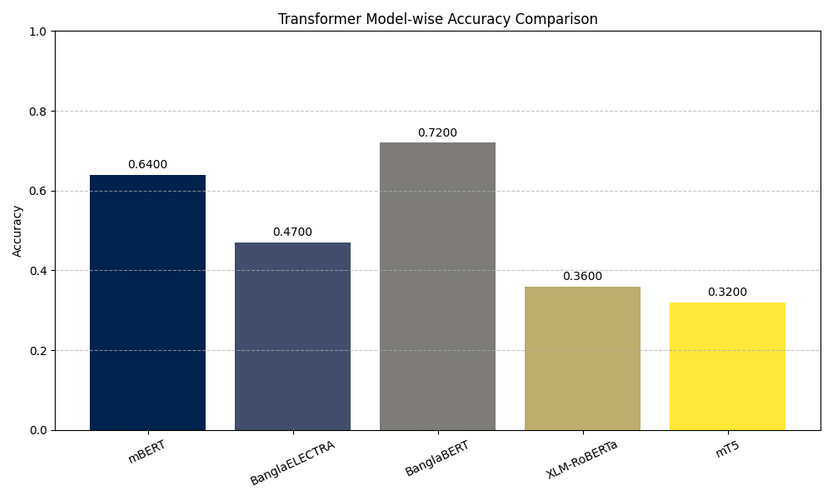
\includegraphics[width=0.38\textwidth]{TL.png}
    \caption{Comparison of transformer-based text models.}
    \label{fig:transformer_comparison}
\end{figure}

\subsubsection{Comparison of Classical ML Models}

Table~\ref{tab:ml_models} presents the performance of classical ML models trained on bag-of-words features. SVM achieves the highest accuracy (0.746), followed by Logistic Regression and Decision Tree (0.73). KNN performs the worst (0.46). Figure~\ref{fig:ml_comparison} shows a visual comparison of all classical ML models.  

\begin{figure}[h]
    \centering
    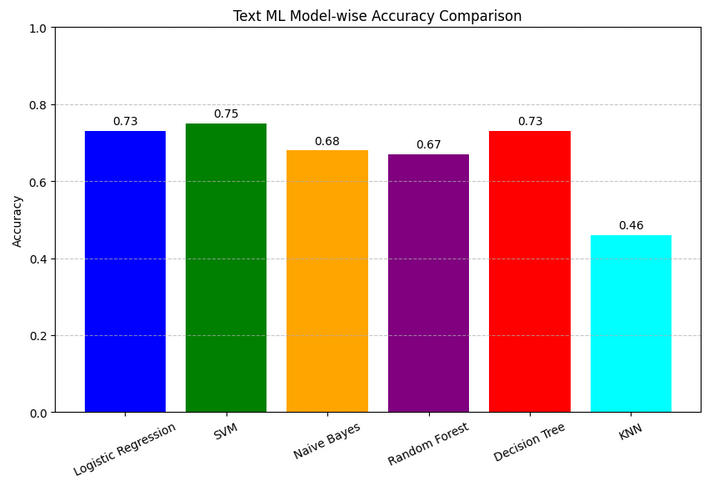
\includegraphics[width=0.38\textwidth]{ML.png}
    \caption{Comparison of classical ML models.}
    \label{fig:ml_comparison}
\end{figure}

\subsection{Image-Based Models}

Table~\ref{tab:image_models} presents the performance of image-based models. ViT achieves the highest accuracy (0.497), demonstrating the advantage of attention-based architectures for visual feature extraction. Figure~\ref{fig:image_comparison} visually compares all image models.  


\begin{table*}[h]
\footnotesize
\centering
\caption{Performance of Baseline Multimodal Models}
\begin{tabular}{|l|c|c|c|c|c|}
\hline
\textbf{Model} & \textbf{Accuracy} & \textbf{Error Rate} & \textbf{Precision} & \textbf{Recall} & \textbf{F1 Score} \\
\hline
CLIP & 0.433 & 0.567 & 0.492 & 0.433 & 0.422 \\
BLIP & 0.467 & 0.533 & 0.464 & 0.467 & 0.447 \\
ALIGN & 0.6 & 0.4 & 0.457 & 0.6 & 0.511 \\
ViLT & 0.467 & 0.533 & 0.556 & 0.467 & 0.486 \\
FLAVA & 0.433 & 0.567 & 0.474 & 0.433 & 0.432 \\
\hline
\end{tabular}
\label{tab:multimodal_models}
\end{table*}




\begin{table*}[h]
\centering
\footnotesize
\caption{Performance of Proposed Multimodal Models}
\begin{tabular}{|l|c|c|c|c|c|}
\hline
\textbf{Proposed Model} & \textbf{Accuracy} & \textbf{Error Rate} & \textbf{Precision} & \textbf{Recall} & \textbf{F1-score} \\
\hline
Proposed Model 1 & 0.6315 & 0.3685 & 0.6448 & 0.6315 & 0.617 \\
Proposed Model 2 & 0.5301 & 0.4699 & 0.5570 & 0.5301 & 0.5261 \\
Proposed Model 3 & 0.4432 & 0.5568 & 0.5040 & 0.4432 & 0.4500 \\
Proposed Model 4 & 0.5239 & 0.4761 & 0.5586 & 0.5239 & 0.5272 \\
Proposed Model 5 & 0.5308 & 0.4692 & 0.5826 & 0.5308 & 0.5282 \\
Proposed Model 6 & 0.4630 & 0.5370 & 0.4728 & 0.4630 & 0.4547 \\
\hline
\end{tabular}
\label{tab:proposed_models_compact}
\end{table*}


\begin{figure}[h]
    \centering
    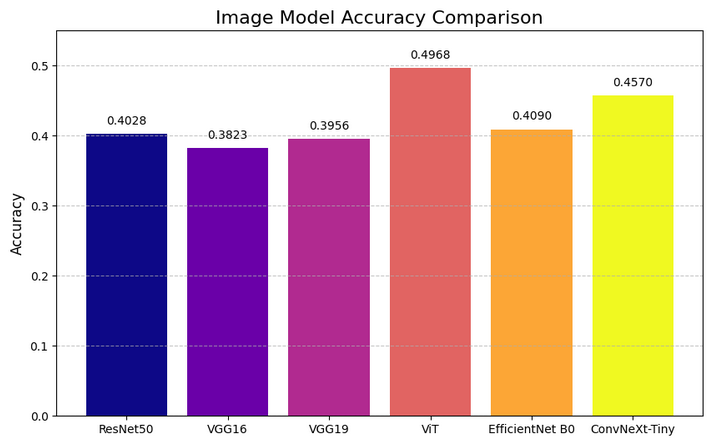
\includegraphics[width=0.38\textwidth]{Image_L.png}
    \caption{Comparison of image-based models.}
    \label{fig:image_comparison}
\end{figure}

\subsection{Baseline Multimodal Models}

Table~\ref{tab:multimodal_models} shows baseline multimodal models. ALIGN achieves the highest accuracy (0.6), showing effective fusion of textual and visual features. Figure~\ref{fig:multimodal_comparison} illustrates the comparison.  

\begin{figure}[h]
    \centering
    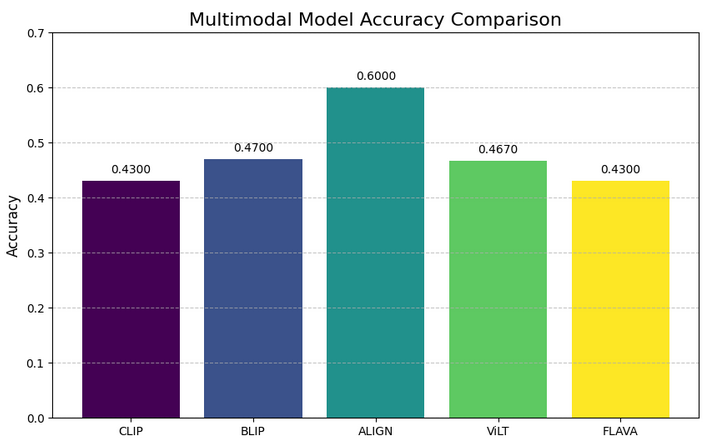
\includegraphics[width=0.38\textwidth]{Multi_L.png}
    \caption{Comparison of baseline multimodal models.}
    \label{fig:multimodal_comparison}
\end{figure}


\subsection{Proposed Multimodal Models}

Table~\ref{tab:proposed_models_compact} presents our six proposed multimodal models. Cross-attention-based fusion (P1) achieves the highest accuracy (0.6315), surpassing the best baseline model (ALIGN: 0.6). Figure~\ref{fig:proposed_comparison} visually compares all six proposed models.  

\begin{figure}[h]
    \centering
    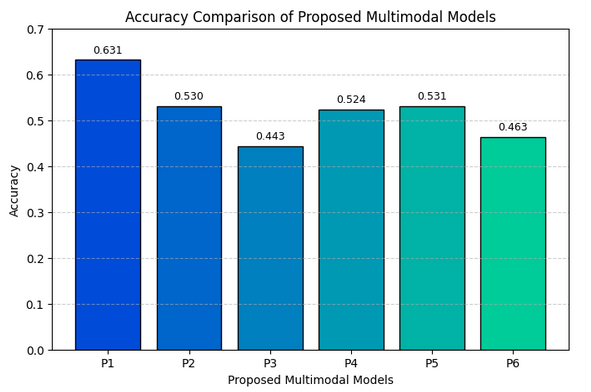
\includegraphics[width=0.38\textwidth]{PL.png}
    \caption{Comparison of the six proposed multimodal models.}
    \label{fig:proposed_comparison}
\end{figure}


\subsection{Analysis of Multimodal vs Text-Only Performance}

ext-only models, such as SVM and BanglaBERT, outperform the proposed multimodal models mainly because the dataset is text-dominant, where sentiment and bias are more clearly expressed in text than in images. Additionally, the relatively small dataset limits the ability of multimodal models to learn effective cross-modal interactions, as these models typically require large-scale data. The visual modality may also contain noisy or weak signals, reducing its contribution to classification. These results indicate that multimodal models do not always ensure better performance, especially in small-scale or text-focused datasets.

Due to computational constraints, standard deviation values are not reported and will be included in future work.


\subsection{Discussion}

The proposed models outperform baseline multimodal architectures by effectively integrating Bangla-specific textual features with visual embeddings. Proposed Model P1 (Hybrid Feature-Level Cross-Attention with Cross-Entropy Loss) achieves the highest accuracy (0.6315), surpassing ALIGN (0.6). Cross-attention allows better alignment of complementary text and image information. Models using simple concatenation, summation, or averaging achieve moderate performance, highlighting the importance of attention-driven fusion. Focal Loss in P2-–P5 improves minority class representation, but cross-attention remains the most effective strategy for Bangla political bias detection. This observation is consistent with prior findings that unimodal text models can outperform multimodal systems in low-resource scenarios. Error analysis reveals that misclassifications often occur in samples with ambiguous or context-dependent expressions. This indicates the need for more context-aware models and larger annotated datasets for improved performance.



\section{Conclusion and Future Work}
In this work, we presented a multimodal deep learning framework for detecting political bias in Bangla news content, leveraging both textual and visual information. By exploring various fusion strategies, including cross-attention, concatenation, summation, averaging, and MFB, we demonstrated that cross-attention-based fusion most effectively captures the inter-modal relationships, achieving an accuracy of 63.2\%. Our study highlights the potential of multimodal approaches for political bias detection and underscores the limitations of existing alignment systems in capturing nuanced biases across text and images. Despite promising results, the study is limited by dataset size and the absence of large-scale multimodal benchmarks, which may affect the generalizability of the findings. For future work, we aim to expand the dataset with more diverse political content and additional modalities such as audio and video. We also plan to explore self-supervised pretraining for multimodal alignment, explainable AI techniques to interpret model decisions. It will focus on expanding the dataset, incorporating transformer-based multimodal architectures, and conducting more extensive evaluations on diverse real-world datasets.



\section*{Limitations}

Our study is limited by the small dataset size and residual class imbalance, which may affect model generalization. Visual data lacks augmentation, and some multilingual transformers underperform on Bangla-specific text. Additionally, current multimodal fusion may not capture all nuanced text-image interactions. Future work should explore larger datasets, improved augmentation, and advanced fusion strategies. Fine-tuning large transformer-based multimodal models on such a small dataset may lead to high variance and unstable performance.




% Bibliography entries for the entire Anthology, followed by custom entries
%\bibliography{anthology,custom}
% Custom bibliography entries only
\bibliography{custom}

\appendix



\end{document}
